%\textbf{Answer all questions} 
%
%\translationbf{Jawab semua soalan}
%\bigskip
\newparten{Answer all questions}

\newpartbm{Jawab semua soalan}
\bigskip 

%\partQuestion{[CO1, PO1]}
\question{}[\label{q1label}]

\listbeginx	% start 1st level question
	\item \label{item:infusion} Infusion pumps are designed to assist in fluids delivery into a patient's body in controlled amounts. Force and pressure sensors are used to ensure the desired amount of fluid is being delivered to the patient and detect occlusion, if any.
	
	\translation{Pam infusi direka bentuk untuk membantu dalam memasukkan cecair ke dalam badan pesakit dengan jumlah yang terkawal. Penderia daya dan tekanan digunakan untuk memastikan jumlah cecair yang dikehendaki dihantar dan mengesan sekatan, sekiranya ada.} 
	
	\listbegin
		\item \label{item:sensor} Suggest a suitable type of sensor to detect force and pressure changes, and justify your suggestion.
		
		\translation{Cadangkan jenis penderia yang sesuai untuk mengesan perubahan daya dan tekanan, dan wajarkan cadangan anda.}
		
		\qmarks{3}	% define marks
		
		\item Elaborate \textbf{TWO (2)} sensor characteristics that are deemed importance for infusion pump as described in Q\ref{q1label}\ref{item:infusion}\ref{item:sensor}
		
		\translation{Huraikan \textbf{DUA (2)} ciri-ciri penderia yang disifatkan penting untuk pam infusi.}
		
		\qmarks{4}

	\listclose % close 2nd level
	
	\item You are given a task to design a capacitive sensor that is able to pass sound frequencies above 25 Hz. For a 1.5 $cm^2$ capacitance sensor, $R$ is 10~\si{\mega\ohm}. (Relative Permitivity $= 8.8854 \times~10^{-12}$)
	
	\translation{Anda diberikan tugasan untuk mereka bentuk penderia kapasitan yang mampu membenarkan frekuensi bunyi lebih 25~Hz. Untuk 1.5~$cm^2$ penderia kapasitan, R adalah \emph{10~\si{\mega\ohm}}. Ketelusan relatif $= 8.854 \times 10^{-12}$,}
	
	\begin{figure}[H] % H means, to put figure here after the code
		\centering
		%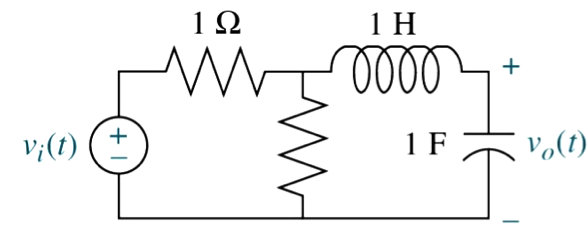
\includegraphics[width=0.5\textwidth]{testfig}
		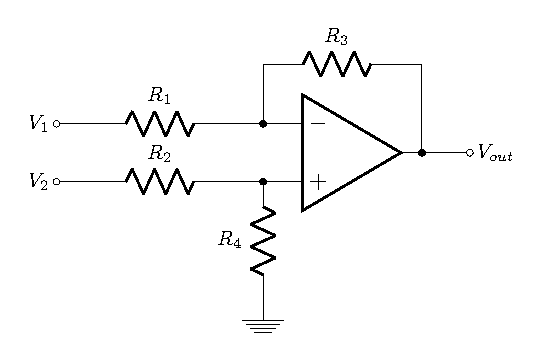
\includegraphics{diffamp}
		\caption{\rajah}
		\label{fig:diffamp}
	\end{figure}
	
\listclose % close 1st level question